% Платформа для разработки "--- основа для приложения,-- пример тире
% его методы для определенных представлений~[10]. -- ссылка на источник
\subsection{Общее описание}
Введем несколько определений.

Процедура доверенной загрузки "--- это процесс загрузки системного программного
обеспечения после выполнения успешной аутентификации оператора изделия и 
исключительно с выбранного учтённого носителя, реализованный в доверенной среде [1].

Доверенная среда "--- это совокупность программно-технических средств и 
коммуникационных ресурсов, для которых однозначно определены состав, архитектура,
алгоритмы функционирования, правила обработки информации и в отношении которой 
верны следующие предположения:
\begin{itemize}
  \item[--] проведены исследования по требованиям нормативных документов по безопасности информации в объёме, согласованном с регулятором;
  \item[--] гарантирована её целостность и неизменность в составе изделия на период эксплуатации за счёт реализации соответствующих программно-технических и организационно-режимных мер.
\end{itemize}


Загрузка операционной системы происходит с жесткого диска, установленного в 
устройстве, такой способ открывает множество возможностей для различных 
хакерских атак и компрометации безопасности системы. Избежать потенциальной "встречи" 
со злоумышленниками можно, используя средства доверенной загрузки (СДЗ).

Средства доверенной загрузки представляют собой решения программно-аппаратные, 
обеспечивающие высокий уровень безопасности еще на самом раннем этапе загрузки 
операционной системы. Основная задача СДЗ "--- контроль целостности программного 
обеспечения и аппаратной конфигурации компьютера перед его запуском. Многие СДЗ 
также выполняют функции средств идентификации и аутентификации пользователей, что 
дополнительно повышает защищенность системы.

Комплексный подход к вопросам доверенной загрузки и применение соответствующих
программно-аппаратных решений позволяет значительно повысить уровень информационной
безопасности компьютерных систем еще до начала их основной эксплуатации, что является 
критически важным в условиях постоянно растущего количество компьютерных угроз.

Особенно актуальна реализация средств доверенной загрузки в критически важных 
системах, таких как банковские терминалы и другие корпоративные устройства. 
Злоумышленники часто пытаются внедрить вредоносное программное обеспечение, 
функционирующее еще до старта основной операционной системы, с целью дальнейшего 
проникновения в корпоративную сеть и компрометации безопасности. Использование 
СДЗ позволяет эффективно противостоять подобным атакам, гарантируя загрузку только
легитимного и проверенного ПО.

\newpage
\subsection{Принципы работы}

В настоящее время был проведен ряд научно-технических работ, по результатам которых
разработан новый подход, лишенный недостатков предыдущих решений. Для реализации 
данного подхода необходимо полное замещение проприетарного программного обеспечения 
BIOS с получением на него исходного кода. Это позволит встроить в BIOS функции 
модуля доверенной загрузки [2].

При этом ПО BIOS будет реализовывать исключительно базовые, минимально необходимые 
функции, достаточные для корректного функционирования процессорной платы с 
установленной операционной системой. Передача управления на загрузчик ОС будет 
осуществляться не BIOS, а самим ПМДЗ, что обеспечит доверенную и максимально 
быструю загрузку всей системы.

\begin{figure}[H]
  \centering
  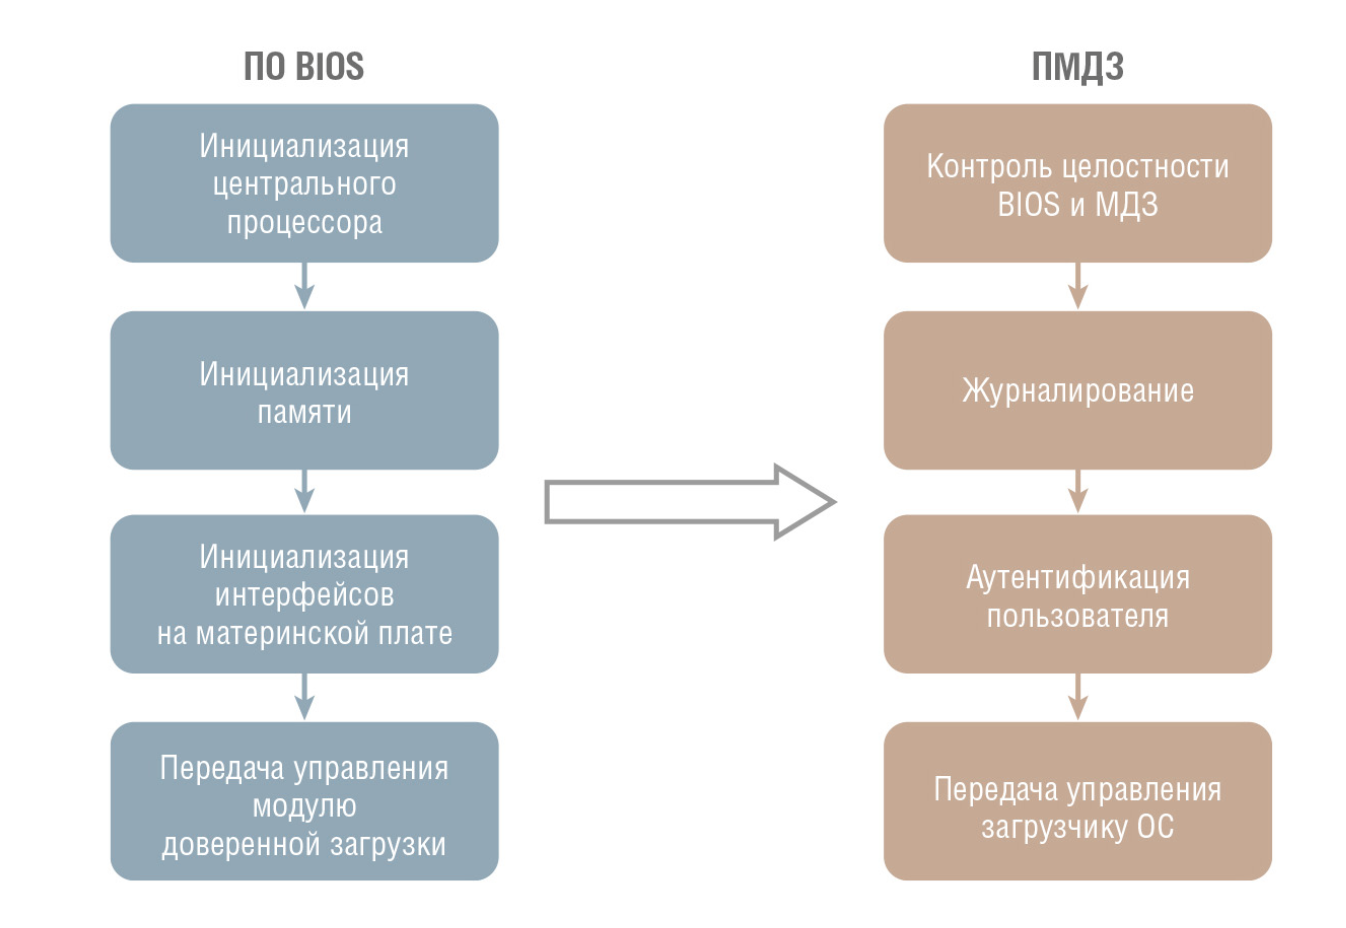
\includegraphics[width=1\textwidth]{pict/8}
  \caption{Общий алгоритм работы ПО BIOS c функциями ПМДЗ}
  \label{fig:55}
\end{figure}

Данный подход позволяет устранить недостатки предыдущих решений и реализовать надежную и эффективную систему доверенной загрузки, интегрированную на низком уровне в базовое программное обеспечение вычислительной платформы.

Модули доверенной загрузки осуществляют верификацию контрольных сумм и других 
характеристик загружаемых данных, сравнивая их с некоторыми уже известными значениями. Таким образом обеспечивается надежный контроль целостности 
программного обеспечения еще до того, как оно будет фактически запущено. Это 
является ключевым фактором защиты от широкого спектра угроз, связанных с загрузкой 
вредоносных модификаций.

Применение средств доверенной загрузки, которые интегрированы в аппаратные платформы или
реализованы в виде отдельных программно-аппаратных устройств, позволяет повысить
уровень информационной безопасности критически важных систем, снизив риски успешных 
атак на этапе загрузки операционной системы.


\newpage
\subsection{Отечественные решения}
На российском рынке представлено множество решений этого класса, каждое из которых
обладает своим набором возможностей и характеристик. Рассмотрим несколько вариантов данных решений:

\subsubsection{«Аккорд-АМДЗ»}
Средство доверенной загрузки уровня платы расширения «Аккорд-АМДЗ» – разработка 
компании «ОКБ САПР» [3]. 

\begin{figure}[H]
  \centering
  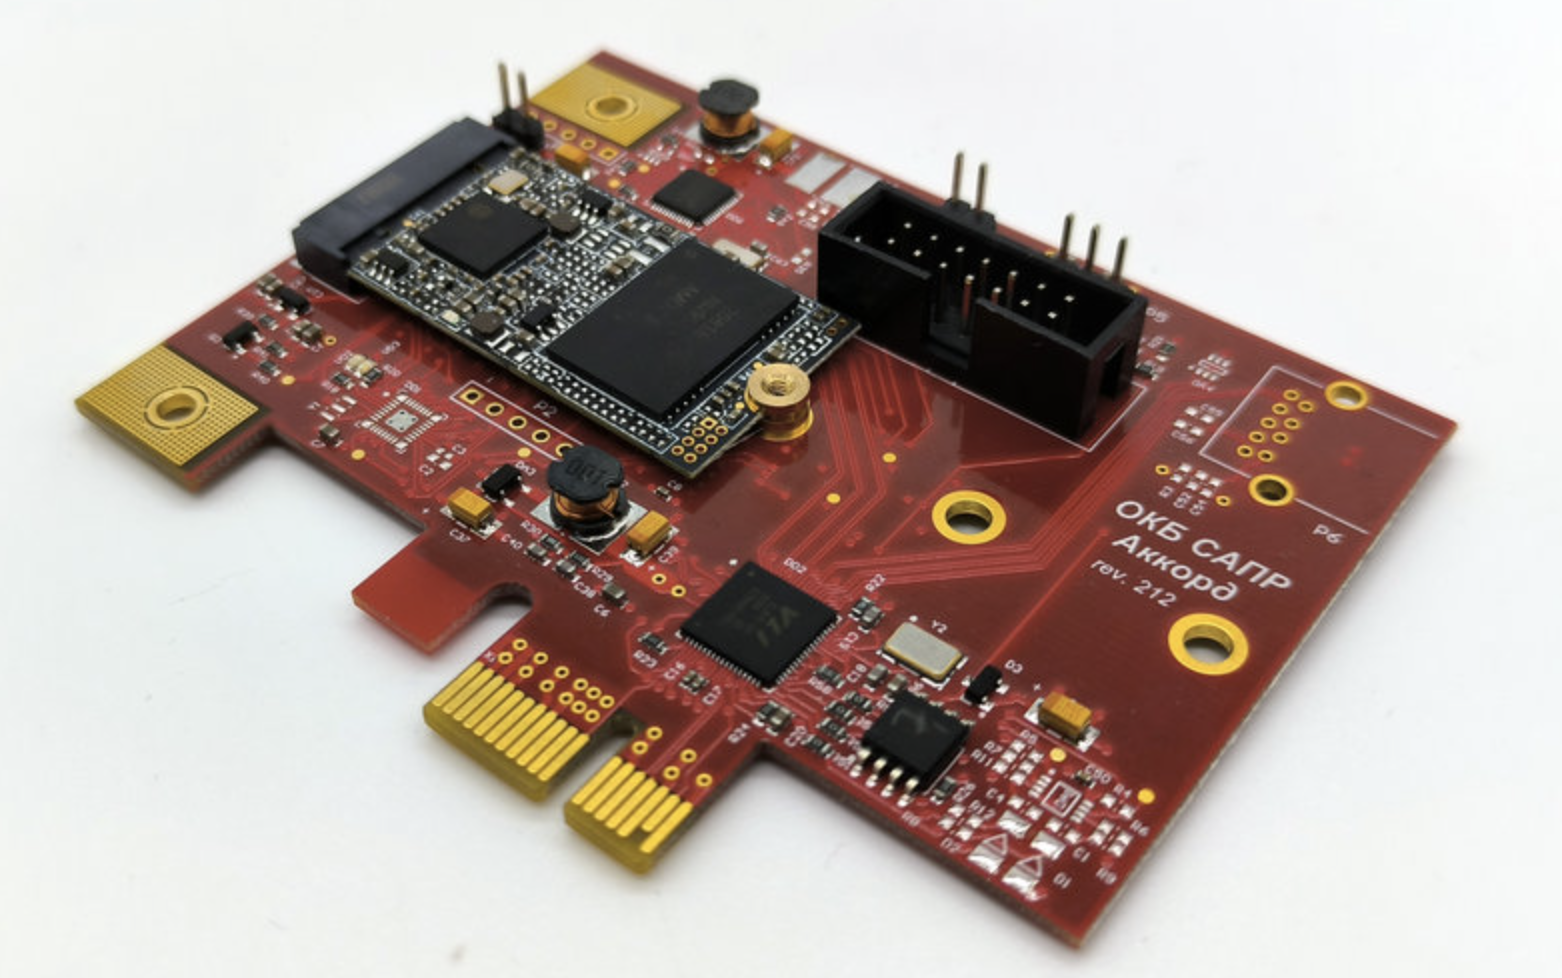
\includegraphics[width=1\textwidth]{pict/17}
  \caption{Аппаратный модуль «Аккорд-АМДЗ»}
  \label{fig:60}
\end{figure}


«Аккорд-АМДЗ» "--- это аппаратный модуль доверенной загрузки
для IBM-совместимых ПК серверов и рабочих станций корпоративной сети. Продукт 
«ОКБ САПР» соответствует концепции резидентного компонента безопасности. Это 
автономное примитивное устройство с защищенной памятью, которое способно влиять 
на архитектуру старта устройства.

Данный защитный комплекс включает в себя специализированный
контроллер с предустановленной операционной средой. Помимо этого, 
СДЗ распространяется вместе с функциональным программным обеспечением. Оба этих
составляющих еще на этапе изготовления становятся частью единого ПО, 
размещенного в энергонезависимой флеш-памяти контроллера.

Комплекс создает доверенную среду для работы программ, обеспечивающих защиту 
на всех шагах (Рис. 3).

\begin{figure}[H]
  \centering
  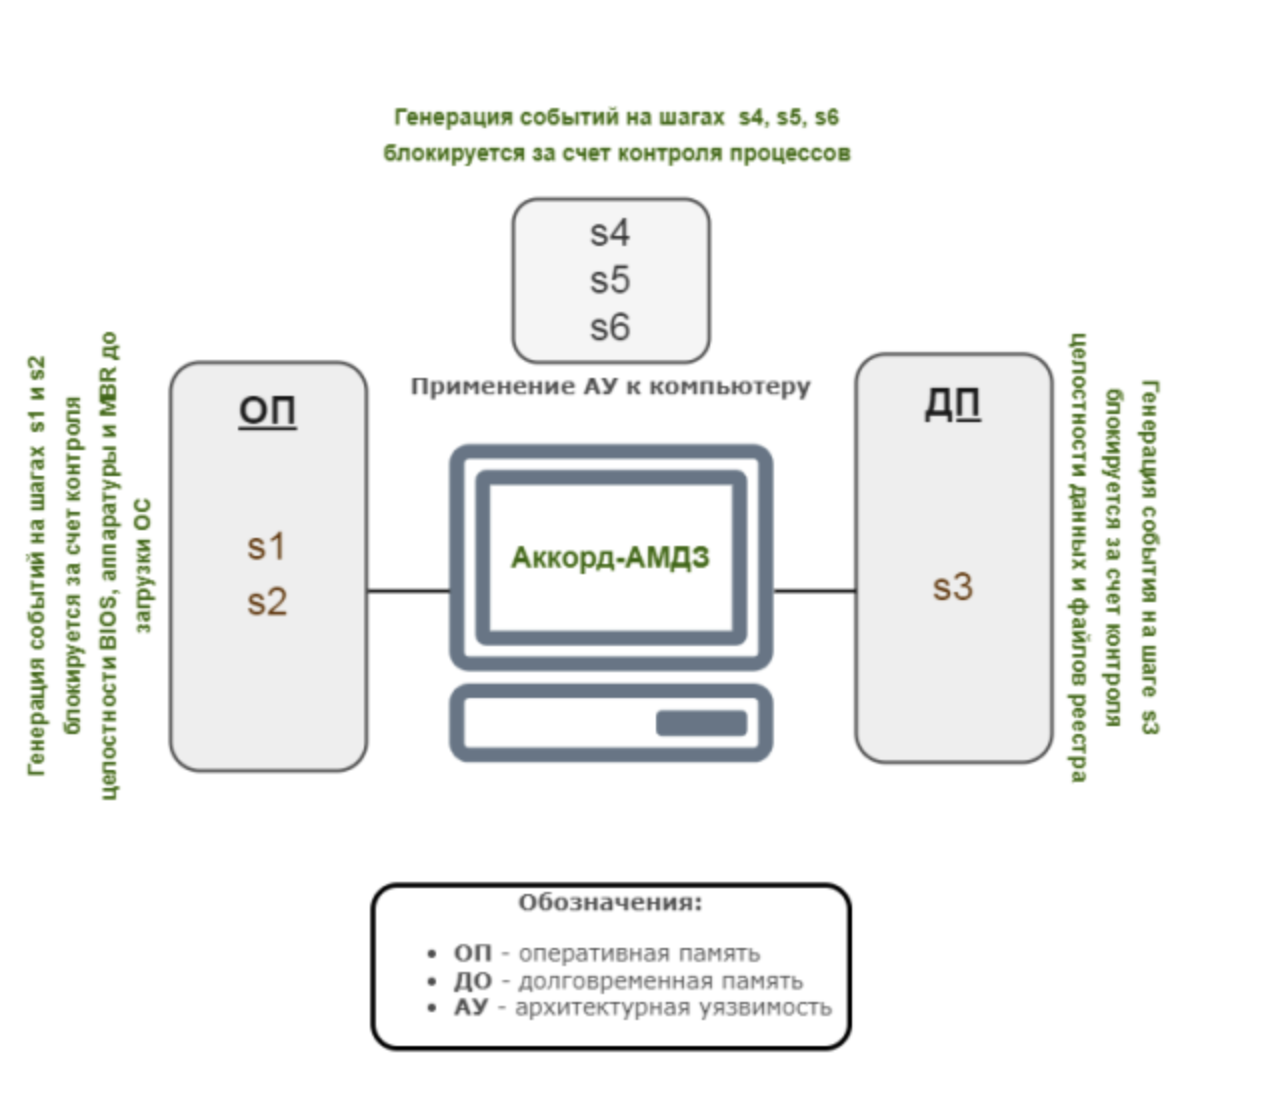
\includegraphics[width=1\textwidth]{pict/9}
  \caption{Работа комплекса}
  \label{fig:56}
\end{figure}


Помимо этого, «Аккорд-АМДЗ» обеспечивает:
\begin{itemize}
  \item[--] защиту ресурсов СВТ от лиц, не допущенных к работе на ней;
  \item[--] аутентификацию пользователей с защитой от раскрытия пароля до загрузки ОС;
  \item[--] блокировку загрузки с внешних носителей;
  \item[--] контроль целостности технических, программных средств и объектов файловых систем, размещенных на динамических дисках;
  \item[--] доверенную загрузку системного и прикладного ПО;
  \item[--] регистрацию контролируемых событий в системном журнале, размещенном в энергонезависимой памяти контроллера;
  \item[--] возможность физической коммутации управляющих сигналов периферийных устройств;
  \item[--] администрирование встроенного ПО комплекса;
  \item[--] регистрацию, сбор, хранение и выдачу данных о событиях, происходящих в СВТ в части системы защиты от несанкционированного доступа.
\end{itemize}

У «Аккорд-АМДЗ» есть сертификаты образцов ФСТЭК. Также это СДЗ входит в реестр отечественного ПО.

\subsubsection{ПАК «Соболь»}
«Соболь» "--- аппаратно-программный модуль доверенной загрузки, функционирующий в среде UEFI. 
Электронный замок «Соболь» предназначен для защиты персональных компьютеров, 
специализированных устройств и серверов в их классическом понимании. Продукт компании 
«Код Безопасности» позволяет вести контроль неизменности файловых систем: NTFS, FAT16,
 FAT32, EXT2, EXT3, EXT4 в операционных системах Linux и Windows [4].

 \begin{figure}[H]
  \centering
  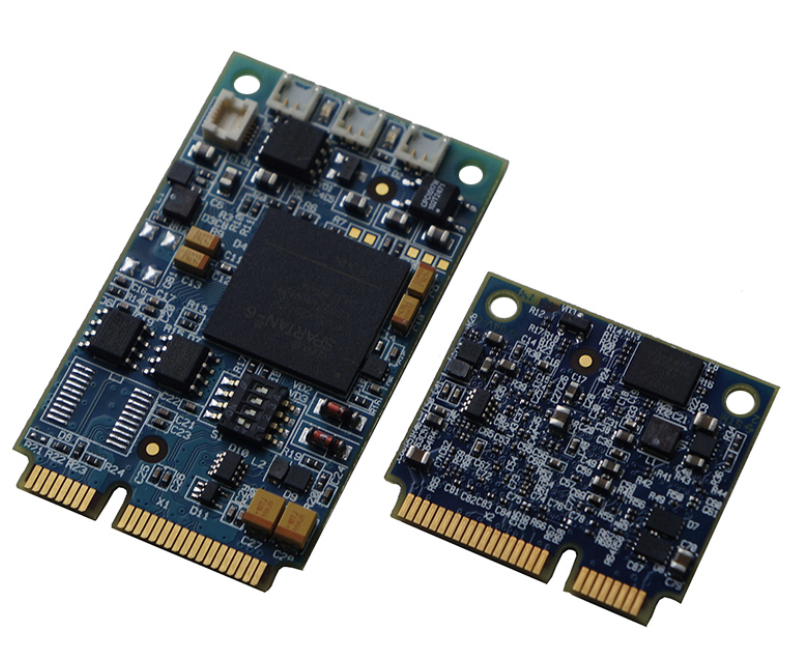
\includegraphics[width=1\textwidth]{pict/15}
  \caption{Аппаратный модуль ПАК «Соболь»}
  \label{fig:61}
\end{figure}


ПАК «Соболь» по заявлениям компании-разработчика создан для решения четырех ключевых задач:
\begin{itemize}
  \item [--] контроль целостности компонентов ИС;
  \item [--] запрет загрузки ОС с внешних носителей;
  \item [--] защита конфиденциальной информации и гостайны в соответствии с требованиями нормативных документов;
  \item [--] защита информации от несанкционированного доступа.
\end{itemize}

\begin{figure}[H]
  \centering
  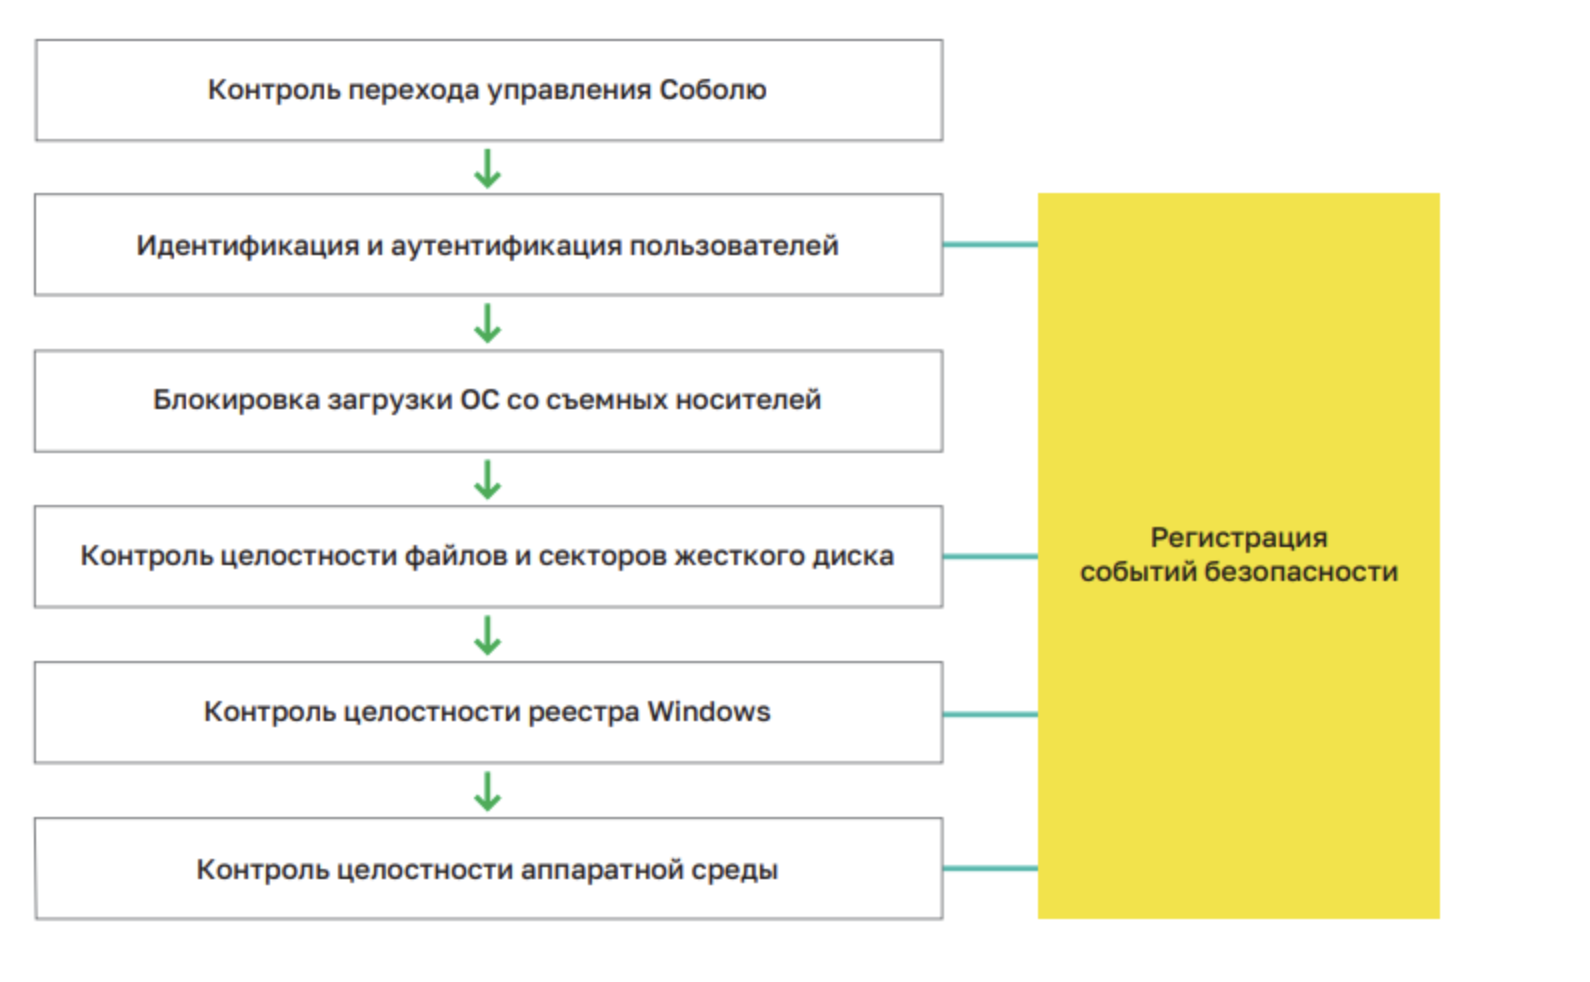
\includegraphics[width=1\textwidth]{pict/11}
  \caption{Принцип работы модуля}
  \label{fig:57}
\end{figure}


Среди интересных преимуществ ПАК «Соболь» можно отметить наличие «сторожевого таймера». 
С его помощью СДЗ блокирует доступ к компьютеру, если управление при его включении 
не передано ПАК «Соболь». Вся информация о попытках входа в систему записывается 
устройством в журнал, который хранится в энергонезависимой памяти. Журнал фиксирует 
не только сам факт входа в систему, но и имя пользователя, предъявление незарегистрированных 
идентификаторов, неправильные вводы пароля, а также дату и время регистрации этих событий.
 Таким образом «Соболь» позволяет компании применить дополнительные меры защиты информации
 при обнаружении несанкционированных попыток входа в систему.

ПАК «Соболь» входит в реестр отечественного ПО. Также продукт имеет сертификаты соответствия
требованиям ФСТЭК и ФСБ.



\subsubsection{Dallas Lock}

Несмотря на американский мотив названия, Dallas Lock "--- разработка российской компании 
«Конфидент». Это средство доверенной загрузки представляет собой плату расширения 
для защиты информации. По заявлению «Конфидент», продукт может защищать сведения вплоть 
до уровня «совершенно секретно». Как и другие решения этого типа Dallas Lock ведет журнал 
и проверяет целостность программно-аппаратной среды до загрузки операционной системы [5].

\begin{figure}[H]
  \centering
  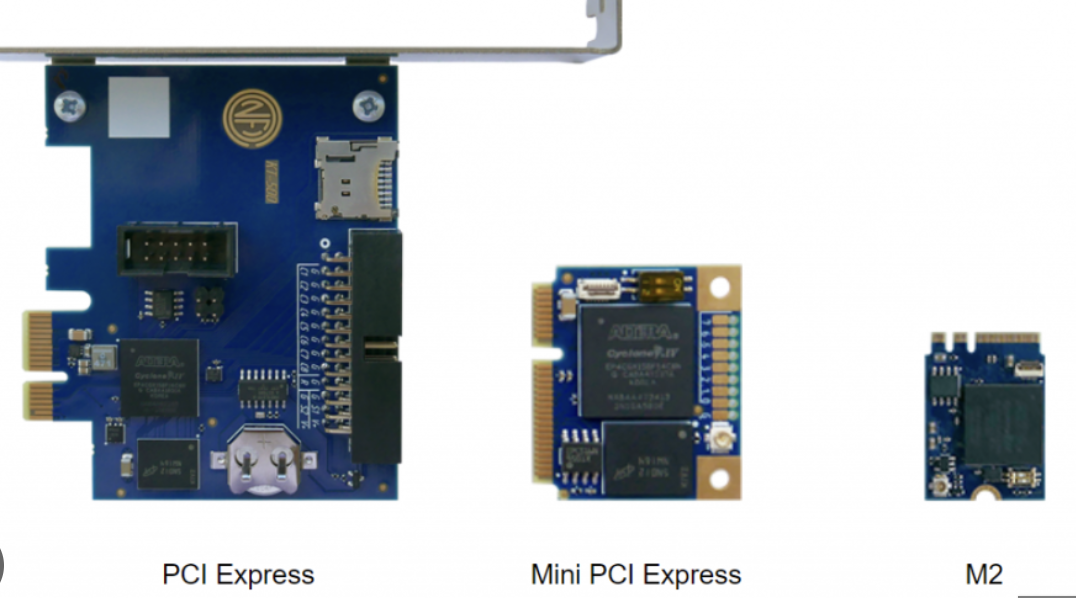
\includegraphics[width=1\textwidth]{pict/14}
  \caption{Аппаратные модули Dallas Lock}
  \label{fig:59}
\end{figure}

Dallas Lock обладает несколькими преимуществами:
\begin{itemize}
  \item[--] администрировать средство доверенной загрузки можно без использования ресурсов загружаемой штатной ОC;
  \item[--] позволяет разграничивать доступ к управлению СДЗ;
  \item[--] СДЗ поддерживает безопасный режим загрузки UEFI;
  \item[--] имеет собственные часы с независимым источником питания;
  \item[--] хранит ключи и служебную информацию в энергонезависимой памяти платы СДЗ;
  \item[--] доступ к СДЗ ограничен после загрузки штатной операционной системы;
\end{itemize}

Решение позволяет использовать двухфакторную аппаратную аутентификацию с популярными USB-ключами и электронными ключами.
\begin{figure}[H]
  \centering
  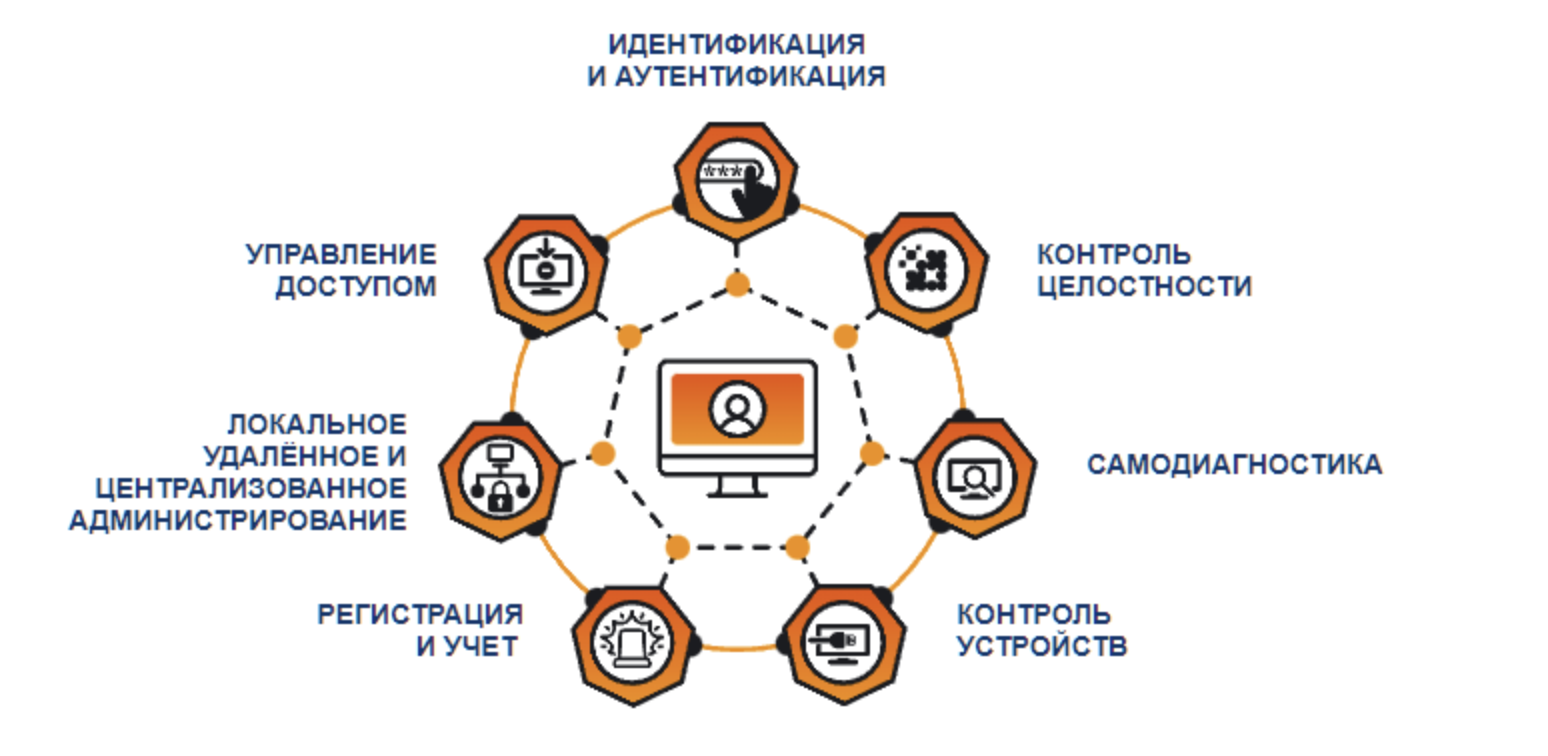
\includegraphics[width=1\textwidth]{pict/12}
  \caption{Комплекс защиты Dallas Lock}
  \label{fig:58}
\end{figure}

СДЗ Dallas Lock входит в реестр отечественного ПО, а также обладает сертификатами ФСТЭК и Минобороны России.

\subsubsection{ViPNet SafeBoot}

Данный продукт разработан российской компанией «ИнфоТеКС». Высокотехнологичный 
программный модуль доверенной загрузки устанавливается в UEFI BIOS. Этот продукт классифицируется как 
СДЗ уровня базовой системы ввода-вывода. ViPNet SafeBoot предназначен для защиты персональных компьютеров, 
мобильных устройств и серверов. Это решение, как и другие, защищает от угрозы несанкционированного 
доступа на этапе загрузки операционной системы [6].

\begin{figure}[H]
  \centering
  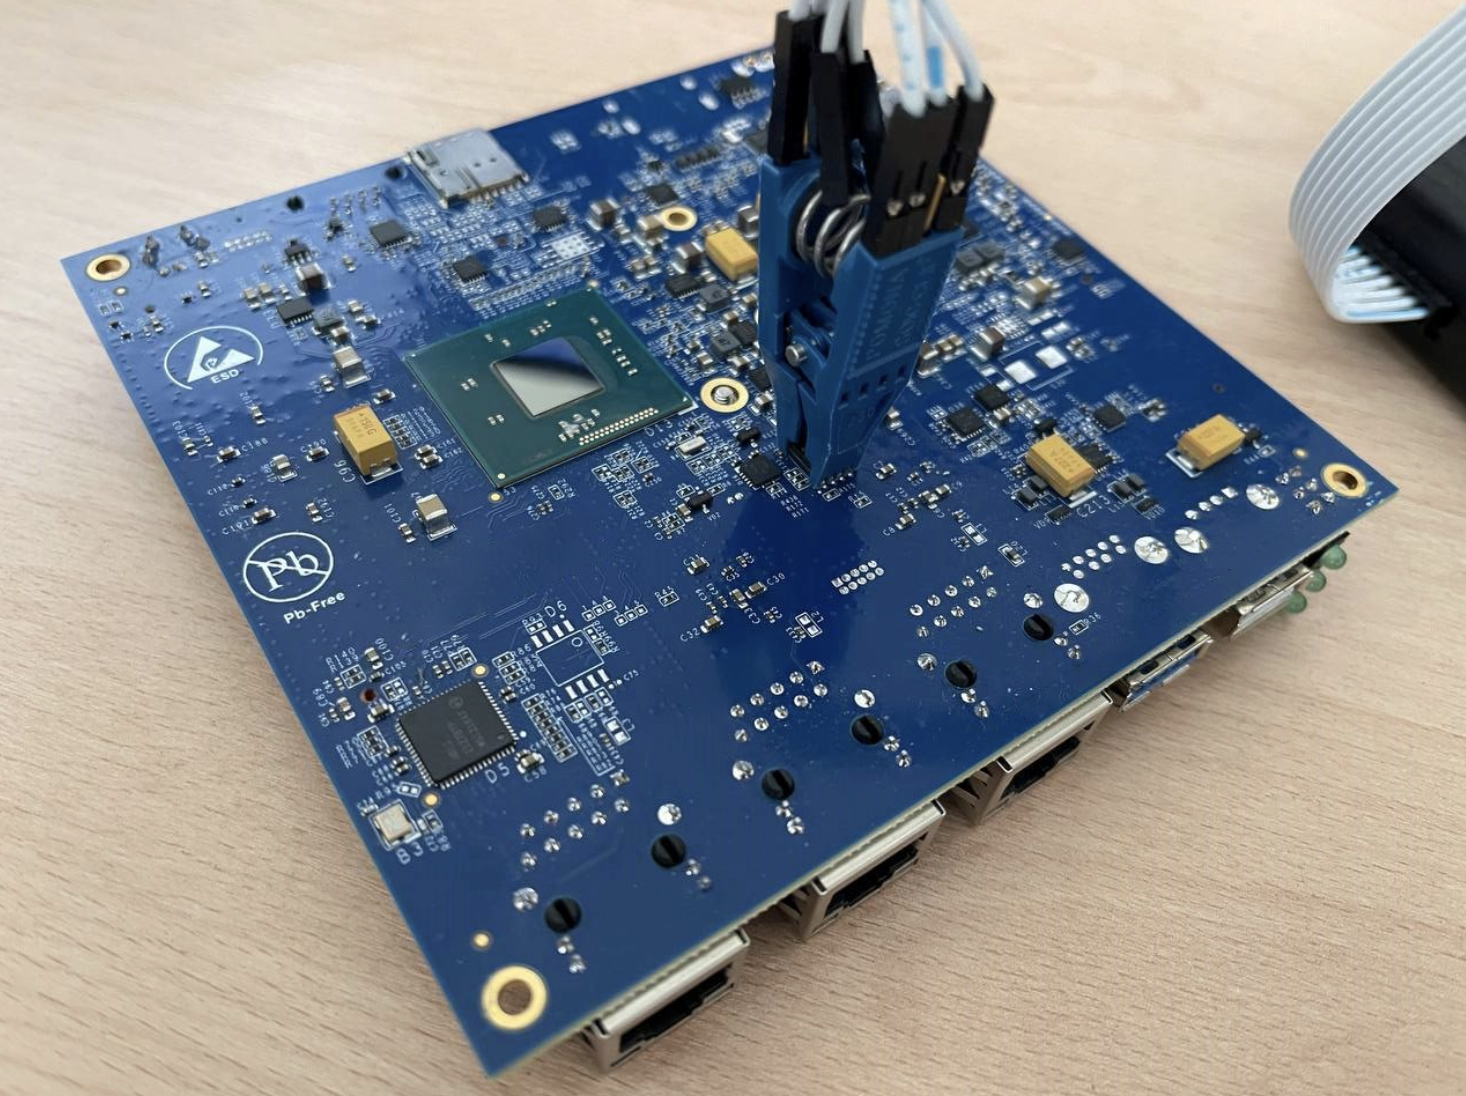
\includegraphics[width=1\textwidth]{pict/13}
  \caption{Аппаратный модуль ViPNet SafeBoot}
  \label{fig:62}
\end{figure}

VipNet SafeBoot обладает несколькими возможностями, среди которых:
\begin{itemize}
  \item [--] авторизация в AD/LDAP;
  \item [--] поддержка SSO для входа в ОС;
  \item [--] защита от вредоносного ПО в BIOS;
  \item [--] ведение журнала событий безопасности;
  \item [--] наличие шаблонов администрирования, позволяющих быстро настроить СДЗ;
  \item [--] защита от обхода и самотестирование;
  \item [--] запрет загрузки с нештатных и внешних носителей;
  \item [--] поддержка двухфакторной аутентификации.
\end{itemize}

Также компания «ИнфоТеКС» среди преимуществ собственного продукта отмечает неизвлекаемость ПМДЗ, 
в отличие от других решений этого класса. VipNet SafeBoot входит в реестр отечественного ПО,
также продукт сертифицирован ФСТЭК России, а значит удовлетворяет требования регуляторов, 
также может быть использовать для построения ИСПДн до У31, ГИС, АСУ ТП и КИИ до 1 класса 
защищенности.


